% Created 2022-10-15 Sat 22:18
% Intended LaTeX compiler: pdflatex
\documentclass[12pt]{article}

%%%% settings when exporting code %%%% 

\usepackage{listings}
\lstdefinestyle{code-small}{
backgroundcolor=\color{white}, % background color for the code block
basicstyle=\ttfamily\small, % font used to display the code
commentstyle=\color[rgb]{0.5,0,0.5}, % color used to display comments in the code
keywordstyle=\color{black}, % color used to highlight certain words in the code
numberstyle=\ttfamily\tiny\color{gray}, % color used to display the line numbers
rulecolor=\color{black}, % color of the frame
stringstyle=\color[rgb]{0,.5,0},  % color used to display strings in the code
breakatwhitespace=false, % sets if automatic breaks should only happen at whitespace
breaklines=true, % sets automatic line breaking
columns=fullflexible,
frame=single, % adds a frame around the code (non,leftline,topline,bottomline,lines,single,shadowbox)
keepspaces=true, % % keeps spaces in text, useful for keeping indentation of code
literate={~}{$\sim$}{1}, % symbol properly display via latex
numbers=none, % where to put the line-numbers; possible values are (none, left, right)
numbersep=10pt, % how far the line-numbers are from the code
showspaces=false,
showstringspaces=false,
stepnumber=1, % the step between two line-numbers. If it's 1, each line will be numbered
tabsize=1,
xleftmargin=0cm,
emph={anova,apply,class,coef,colnames,colNames,colSums,dim,dcast,for,ggplot,head,if,ifelse,is.na,lapply,list.files,library,logLik,melt,plot,require,rowSums,sapply,setcolorder,setkey,str,summary,tapply},
aboveskip = \medskipamount, % define the space above displayed listings.
belowskip = \medskipamount, % define the space above displayed listings.
lineskip = 0pt} % specifies additional space between lines in listings
\lstset{style=code-small}
%%%% packages %%%%%

\usepackage[utf8]{inputenc}
\usepackage[T1]{fontenc}
\usepackage{lmodern}
\usepackage{textcomp}
\usepackage{color}
\usepackage{graphicx}
\usepackage{grffile}
\usepackage{wrapfig}
\usepackage{rotating}
\usepackage{longtable}
\usepackage{multirow}
\usepackage{multicol}
\usepackage{changes}
\usepackage{pdflscape}
\usepackage{geometry}
\usepackage[normalem]{ulem}
\usepackage{amssymb}
\usepackage{amsmath}
\usepackage{amsfonts}
\usepackage{dsfont}
\usepackage{array}
\usepackage{ifthen}
\usepackage{hyperref}
\usepackage{natbib}
\pagestyle{empty} % no page numbering
\usepackage[french, english]{babel}
\newcommand{\Rlogo}{\textbf{\textsf{R}}}
\newcommand{\Cpp}{C\nolinebreak\hspace{-.05em}\raisebox{.4ex}{\tiny\bf +}\nolinebreak\hspace{-.10em}\raisebox{.4ex}{\tiny\bf +}}
\usepackage{eurosym} % euro symbol
\usepackage{titlesec}
\titleformat{\section}{\large}{\thesection}{1em}{}
\titlespacing*{\section}{0pt}{0.25\baselineskip}{0.25\baselineskip}
\geometry{
left=20mm,
right=20mm,
top=20mm,
bottom=20mm
}
\hypersetup{
citecolor=[rgb]{0,0.5,0},
urlcolor=[rgb]{0,0,0.5},
linkcolor=[rgb]{0,0,0.5},
}
\RequirePackage{setspace} % to modify the space between lines - incompatible with footnote in beamer
\renewcommand{\baselinestretch}{1.1}
\usepackage{framed}
\usepackage{tocloft}
\newlength{\outerbordwidth}
\raggedbottom
\raggedright
\setlength{\outerbordwidth}{3pt}  % Width of border outside of title bars
\definecolor{shadecolor}{gray}{0.75}  % Outer background color of title bars (0 = black, 1 = white)
\definecolor{shadecolorB}{gray}{0.93}  % Inner background color of title bars
\usepackage{mdframed}
\newcommand{\resitem}[1]{\item #1 \vspace{-2pt}}
\newcommand{\resheading}[1]{
\vspace{8pt}
\parbox{\textwidth}{\setlength{\FrameSep}{\outerbordwidth}
\begin{shaded}
\setlength{\fboxsep}{0pt}\framebox[\textwidth][l]{\setlength{\fboxsep}{4pt}\fcolorbox{shadecolorB}{shadecolorB}{\textbf{\sffamily{\mbox{~}\makebox[6.762in][l]{\large #1} \vphantom{p\^{E}}}}}}
\end{shaded}
}\vspace{-5pt}
}
\newcommand{\ressubheading}[4]{
\begin{tabular*}{6.5in}{l@{\cftdotfill{\cftsecdotsep}\extracolsep{\fill}}r}
\textbf{#1} & #2 \\
\textit{#3} & \textit{#4} \\
\end{tabular*}\vspace{-6pt}}
\usepackage{bibentry}
\nobibliography*
\newcommand{\myname}[1]{\textbf{#1}}
\usepackage{url}
\usepackage{enumitem}
\date{\today}
\title{}
\hypersetup{
 colorlinks=true,
 pdfauthor={Brice Ozenne},
 pdftitle={},
 pdfkeywords={},
 pdfsubject={},
 pdfcreator={Emacs 26.3 (Org mode 9.4.6)},
 pdflang={English}
 }
\begin{document}

\begin{tabular*}{7in}{l@{\extracolsep{\fill}}r}
	\textbf{\Large Brice Ozenne} & \textbf{\today} \\
\end{tabular*}

\bigskip

\begin{minipage}{0.2\linewidth}
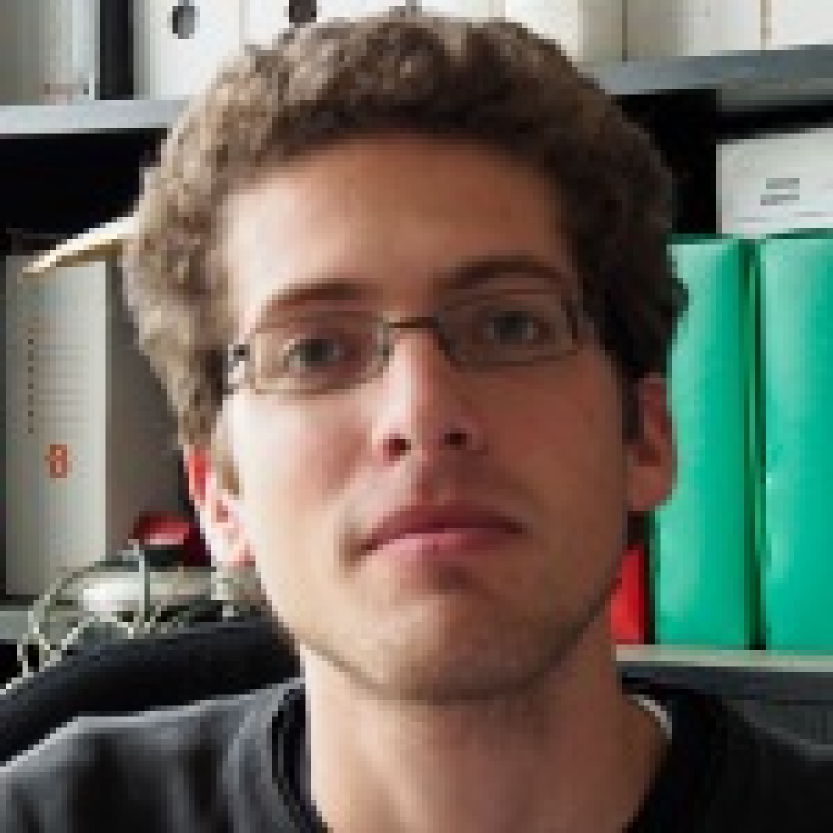
\includegraphics[width=\linewidth]{photoId.png}
\end{minipage}
\begin{minipage}{0.75\linewidth}
\begin{tabular*}{7in}{ll@{ }l}
	Nationality&:& french  \\
	Date of birth&:& February 8, 1990  \\
	Personal email&:& \url{brice.mh.ozenne@gmail.com} \\ 
	Personal phone number&:& (+45) 52 328 128 \\ 
        Personal address&:& Nordre Teglkaj 18, 5 t.h., 2450 Copenhagen SV, Denmark \\
        Personal Website&:& \url{https://bozenne.github.io/} \\
        Github&:& \url{https://github.com/bozenne/} \\
\end{tabular*}
\end{minipage}

\bigskip

\resheading{Current position}
\begin{tabular}{l@{ }l}
	November 2015- Now:& \textbf{Assistant professor in biostatistics} with a shared position between \\ [2mm]
	& - a research unit in biostatistics \\
	& \href{https://biostat.ku.dk/staff_/?pure=en/persons/540231}{Section of Biostatistics}, University of Copenhagen \\
	& \O{}ster Farimagsgade 5, 1014 Copenhagen, Denmark \\ [2mm]
	& - a research unit in neuroscience \\
	& \href{https://nru.dk/index.php/staff-list/post-docs/110-brice-ozenne}{Neurobiology Research Unit} \\
	& Copenhagen University Hospital, Rigshospitalet \\
	& Building 6931, Blegdamsvej 9, DK-2100 Copenhagen, Denmark \\ [2mm]
      & where I do research in biostatistics along with a consulting activity in statistics \\
      & and some teaching.
\end{tabular}

\bigskip
My research work is organized around three topics:
\begin{itemize}
\item the development of \textbf{multivariate models} for data analysis in
neuroscience, mainly latent variable models (LVM) and mixed models (LMM) - see publications
\cite{ebert2019molecular,stenbaek2017brain,fisher2017bdnf}. From a
methodological point of view, I study how to perform statistical
\textbf{estimation and inference in small samples} \citep{ozenne2020small} as
well as efficient corrections for \textbf{multiple testing}
\citep{ozenne2022controlling}. These developments are available in the
R packages \texttt{lavaSearch2} (LVM) and \texttt{LMMstar} (LMM).

\item the analysis of registry data in presence of \textbf{right-censoring},
\textbf{competing risks}, and \textbf{confounding} \textbf{competing risks}. A typical
application is the comparison of preventive treatments of
cardiovascular diseases
\citep{staerk2016ischaemic,staerk2017resumption,staerk2018standard}. Based
on the \textbf{semi-parametric theory}, I have developped a robust
estimator of the average treatment effect and derived its asymptotic
distribution via its influence function
\citep{ozenne2020estimation}. This has been implemented in the \texttt{ate}
function of the \texttt{riskRegression} R package.
\end{itemize}

\clearpage

\begin{itemize}
\item the extension of \textbf{generalized pairwise comparisons} (GPC) to
right-censoring \citep{peron2016extension}. GPC is a method able to
handle multiple and heterogeneous endpoints which is especially
relevant to assess the benefit-risk balance of a treatment. A
typical application is the evaluation of chemotherapies where
jointly considering gains in survival and side effects is critical
\citep{peron2016net,peron2016assessment}. I am now working on deriving
the asymptotic distribution of some of the estimators implemented in
the \texttt{BuyseTest} using the U-statistique theory.
\end{itemize}

\bigskip

\section*{\emph{Other domains of interest in statistics:}}
\label{sec:org161f5c0}
\begin{itemize}
\item Smoothing splines and functional data analysis
\item Causal inference and dynamic treatment regimes
\item Post-selection inference
\end{itemize}
\resheading{Skills}

\section*{\emph{Language}}
\label{sec:org90b0f12}
French (native language), english (fluent), danish (intermediate),
basics in italian.

\section*{\emph{Software}}
\label{sec:org9168a13}
Proficient in \Rlogo{}, \LaTeX{} and \href{https://orgmode.org/}{orgmode}. \\ 
Basic knowledge but common use of \Cpp{}, lisp (for \href{https://www.gnu.org/software/emacs/}{GNU Emacs}) and
git/github (via \href{https://magit.vc/}{magit}).
\resheading{Education and research carrier}
\begin{tabular}{l@{ }l}
2020 - 2015 : & Post-doc in biostatistics with a shared positive between: \\
              & \emph{University of Copenhagen}: researcher and teacher at the Graduate School \\
              & of Health and Medical Sciences \\ 
              & \emph{Copenhagen University Hospital}: consultant and leader of the data analysis workpackage \\ 
              & of the \href{https://np.nru.dk/}{Neuropharm} project  \\ 
              & Development of LVM for analysing brain data (\texttt{lavaSearch2} package) and \\
              & robust estimators of treatment effect for registry data analysis (R package \texttt{riskRegression}) \\ [3mm]
2012 - 2015 : & Ph.D. in biostatistics, University Lyon 1, Lyon, France. \\
              & Thesis Title: \href{https://tel.archives-ouvertes.fr/tel-01233049/document}{Statistical modelling for the prognosis of stroke patients.} \\ 
              & Advisor: Pr. Delphine Maucort-Boulch and Pr. Norbert Nighoghossian \\ [3mm]
2011 - 2012 : & Master’s degree in biostatistics (\href{https://clarolineconnect.univ-lyon1.fr/icap_website/299/5381}{M2 B3S}), University lyon, Lyon, France. \\ 
              & Carried out in double degree with the École Centrale de Lyon. \\ [3mm]
2009 - 2012 : & Engineering diploma from the École Centrale de Lyon, Lyon, France. \\
              & Erasmus at Politecnico di Milano (2nd semester 2011). \\
\end{tabular}

\resheading{Teaching and supervision}

Teaching (L : lecture, PC : practical classes)
\begin{tabular}{l@{ }l}
2015 - 2020 : & \href{http://publicifsv.sund.ku.dk/~jufo/RepeatedMeasures2019.html}{Statistical analysis of repeated measurements} for Phd students in medical sciences (18h, PC). \\ 
2016 - 2017 : & Structural Equation Models for Master students in statistics (2h, L). \\
2014 - 2015 : & \href{http://mastersantepublique.univ-lyon1.fr/webapp/website/website.html?id=3124911&pageId=215839}{Survival Analysis} for Master students in public health (18h, PC).\\
2013 - 2015 : & \href{http://mastersantepublique.univ-lyon1.fr/webapp/website/website.html?id=3124911&pageId=215839}{Bayesian statistics} for Master students in public health (6h, PC).\\
\end{tabular}

\bigskip

Pedagogical talks for researchers in neuroscience on specific
statistical tools/issues:
\begin{itemize}
\item \href{https://bozenne.github.io/doc/Talks/2017-XNRU-power.pdf}{Do we need more power?} (\href{https://www.nru.dk/images/News/NeurobiologyResearchUnit-Christmas-symposium2017.pdf}{NRU Christmas Symposium 2017}).
\item \href{https://bozenne.github.io/doc/Talks/2018-XNRU-DAGs.pdf}{To adjust or not adjust, that is the question} (NRU Christmas Symposium 2018).
\item \href{https://bozenne.github.io/doc/Talks/2019-XNRU-multcomp.pdf}{A refresher on multiple comparisons}? (\href{https://nru.dk/index.php/news-menu/279-nru-christimas-symposium-2019}{NRU Christmas Symposium 2019}).
\end{itemize}

\bigskip

Co-supervision of \textbf{master 2} student: 

\medskip

\begin{tabular}{l@{ }l@{ }l}
2014 &:& Ceren Tozlu \\
\multicolumn{3}{l}{Comparison of classification methods for tissue outcome after ischemic stroke \citep{tozlu2019comparison}.} \\ [3mm]
2019 &:& Alice Brouquet-Laglaire \\
\multicolumn{3}{l}{Comparison of inference methods for generalized pairwise comparisons.} \\ [3mm]
\end{tabular}

\resheading{Grants}
\begin{tabular}{l@{ }l}
2017-2019: MARIE CURIE Individual Fellowships (200 000\euro, EU H2020-MSCA-IF-2016 746850) \\
2017-2020: Lundbeck Fellowships (140 000\euro, R231-2016-3236) \\
\end{tabular}

\clearpage

\resheading{Scientific output \hfill \href{https://scholar.google.com/citations?user=rJMNP7YAAAAJ&hl=fr}{link google scholar}}
\section*{\emph{Publications (methodological)}}
\label{sec:orgc2fc4ac}

Published:
\begin{enumerate}
   \item \bibentry{scheike2022efficient}
   \item \bibentry{ozenne2022controlling}
   \item \bibentry{ozenne2021asymptotic}
   \item \bibentry{peron2021correcting}
   \item \bibentry{cantagallo2021new}
   \item \bibentry{ozenne2020small}
   \item \bibentry{verbeeck2020evaluation}
   \item \bibentry{ozenne2020estimation}
   \item \bibentry{norgaard2019preprocessing}
   \item \bibentry{ozenne2017riskregression}
   \item \bibentry{peron2016extension}
   \item \bibentry{ozenne2015precision}
   \item \bibentry{ozenne2015spatially}
 \end{enumerate}

\pagebreak[3]

\resheading{Software development}

Packages for the \href{https://www.r-project.org/}{R} software:
\begin{itemize}
\item \textbf{BuyseTest} (author and maintainer): implementation of generalized
pairwise comparisons, including recent developments to handle
right-censoring
\citep{peron2016extension,peron2021correcting}. Available on \href{https://cran.r-project.org/web/packages/BuyseTest/index.html}{CRAN} and on
\href{https://github.com/bozenne/BuyseTest}{Github}.

\item \textbf{lavaSearch2} (author and maintainer): Inference and diagnostic
tools for latent variable models.  Methodology described in
\citep{ozenne2020small} and \citep{ozenne2022controlling}. Available on
\href{https://cran.r-project.org/web/packages/lavaSearch2/index.html}{CRAN} and on \href{https://github.com/bozenne/lavaSearch2}{Github}. .

\item \textbf{LMMstar} (author and maintainer) : linear mixed model via
covariance structure (marginal formulation). Inference in small
sample, test linear and non-linear combinations of parameters,
multiple comparisons adjustment. Disponible sur le \href{https://cran.r-project.org/web/packages/LMMstar/index.html}{CRAN} et sur
\href{https://github.com/bozenne/LMMstar}{Github}. .

\item \textbf{riskRegression} (contributor): computation of absolute risks and
average treatment effects. Methodology described in
\citep{ozenne2017riskregression} and
\citep{ozenne2020estimation}. Available on \href{https://cran.r-project.org/web/packages/riskRegression/index.html}{CRAN} and on \href{https://github.com/tagteam/riskRegression}{Github}.
\end{itemize}

\clearpage

Package for \href{https://www.gnu.org/software/emacs/}{emacs}:
\begin{itemize}
\item \textbf{emacs-config} (author and maintainer) : Configuration files for
emacs to ease the interaction with
R/C++/orgmode/latex/git. Disponible on \href{https://github.com/bozenne/emacs-config}{Github}.
\end{itemize}

\pagebreak[3]

\section*{\emph{Publications (clinical applications)}}
\label{sec:org7189838}

\begin{enumerate}[resume]
   \item \bibentry{nasser2022reliability}
   \item \bibentry{armand2022brain}
   \item \bibentry{kohler2022concurrent}
   \item \bibentry{armand2022acute}
   \item \bibentry{armand2022brain}
   \item \bibentry{fisher2022emotional}
   \item \bibentry{beaman2022blood}
   \item \bibentry{drummond2022psilocybin}
   \item \bibentry{larsen2022impact}
   \item \bibentry{mcculloch2022lasting}
   \item \bibentry{ip2021eeg}
   \item \bibentry{madsen2021psilocybin}
   \item \bibentry{joergensen2021default}
   \item \bibentry{brandt2021reward}
   \item \bibentry{dea2021brain}
   \item \bibentry{ip2021pretreatement}
   \item \bibentry{hoghe2021MAMA}
   \item \bibentry{raval2021single}
   \item \bibentry{hogsted2021stress}
   \item \bibentry{donovan2021effects}
   \item \bibentry{lee2020absolute}
   \item \bibentry{hansen2020visual}
   \item \bibentry{spies2020common}
   \item \bibentry{larsen2020oral}
   \item \bibentry{thystrup2020severity}
   \item \bibentry{dam2020hot}x
   \item \bibentry{hjordt2020psychometric}
   \item \bibentry{beliveau2020structure}
   \item \bibentry{madsen2020single}
   \item \bibentry{ozenne2019individualized}
   \item \bibentry{ebert2019molecular}
   \item \bibentry{madsen2019psychedelic}
   \item \bibentry{tozlu2019comparison}
   \item \bibentry{ip2018pre}
   \item \bibentry{borgsted2018amygdala}
   \item \bibentry{hjordt2018self}
   \item \bibentry{foged2018verbal}
   \item \bibentry{staerk2018standard}
   \item \bibentry{hjordt2017season}
   \item \bibentry{beliveau2017high}
   \item \bibentry{stenbaek2017brain}
   \item \bibentry{staerk2017resumption}
   \item \bibentry{fisher2017bdnf}
   \item \bibentry{foged2017safety}
   \item \bibentry{peron2016net}
   \item \bibentry{staerk2016ischaemic}
   \item \bibentry{peron2016assessment}
   \item \bibentry{ozenne2015evaluation}
   \item \bibentry{hermitte2013very}
 \end{enumerate}

\pagebreak[3]
\resheading{Peer review}
I have reviewed papers for Biometrics, Statistics in Medicine, and the
International Journal of Biostatistics.


\resheading{Oral communications}
Oral presentation at international conferences: 

\medskip

\begin{tabular}{l@{ }l@{ }l}
2014 &:& Lesion Segmentation using a Spatially Regularized Mixture Model \\
&& \href{http://conferences.nib.si/AS2014/default.htm}{Applied Statistics}, Ribno, Slovenia \hfill (\href{https://bozenne.github.io/doc/Talks/2014-Applied_statistics-Lesion_Segmentation.pdf}{slides}) \\ [3mm]
2015 &:& MRIaggr : un package pour la gestion et le traitement de données multivariées d'imagerie\\
&& \href{https://r2015-grenoble.sciencesconf.org/66037}{Rencontres R, Grenoble, France}  \hfill   (\href{https://bozenne.github.io/doc/Talks/2015-R-MRIaggr.pdf}{slides})  \\ [3mm]
2016 &:& Penalized latent variable models  \\
&& \href{http://cmstatistics.org/RegistrationsV2/COMPSTAT2016/viewSubmission.php?in=440&token=29584n1s18p97n65o7p1r5n36sopq0n4}{Computational statistics}, Oviedo, Spain \hfill (\href{https://bozenne.github.io/doc/Talks/2016-Compstat-pLVM.pdf}{slides}) \\ [3mm]
2017 &:& Assessing treatment effects on registry data in presence of competing risks \\ 
&& ISCB, Vigo, Spain \hfill (\href{https://bozenne.github.io/doc/Talks/2017-ISCB-ate.pdf}{slides}) \\ [3mm]
2019 &:& Generalized pairwise comparisons for right-censored time to event outcomes \\
&& \href{https://publicifsv.sund.ku.dk/~safjr2019/}{Survival analysis for junior researcher}, Copenhagen, Denmark \hfill (\href{https://bozenne.github.io/doc/Talks/2019-prezSAfJR-GPC.pdf}{slides}) \\ [3mm]
2019 &:& Multiple testing in latent variable models \\
&& \href{https://kuleuvencongres.be/iscb40/}{ISCB}, Leuven, Belgium \hfill (\href{https://bozenne.github.io/doc/Talks/2019-ISCB-multcomp_LVM.pdf}{slides}) \\
\end{tabular}

\bigskip

Invited speaker at an internation conference: 

\medskip

\begin{tabular}{l@{ }l@{ }l}
2019 &:& Region-Based and Voxel-Wise Analysis of Medical Images Using Latent Variables \\
&& \href{https://events.razzby.com/nbbc19/}{7th NBBC}, Vilnius, Lithuania \\
december 2020 &:& Robust estimation of the average treatment effects in presence of right-censoring \\
&& and competing risks \\
&& \href{http://www.cmstatistics.org/conferences.php}{CMStatistics}, London, England \\
\end{tabular}

\bigskip

Chairman at international conferences:

\medskip

\begin{tabular}{l@{ }l@{ }l}
2019 &:& Mathematical Statistics \\
&& \href{https://publicifsv.sund.ku.dk/~safjr2019/}{Survival analysis for junior researcher}, Copenhagen, Denmark
\end{tabular}

\bigskip

Organisation of a workshop:
\begin{tabular}{l@{ }l@{ }l}
2021 &:& Analysis of repeated measurements with mixed models using the R package LMMstar (1h+3h) \\
&& Methods Week, Karolinska institute, Stockholm, Suède
\end{tabular}

\bibliographystyle{plainnat}

\nobibliography{publicationBO}
\end{document}